%Präambel
\documentclass[fontsize=12, a4aper]{scrartcl}
\usepackage{setspace}
\onehalfspacing
\setcounter{secnumdepth}{4}

\usepackage{cite}
\usepackage{url}
\usepackage[english, ngerman]{babel}
\usepackage{mwe}
\usepackage{newfloat}
\usepackage[utf8]{inputenc}
\usepackage[autostyle=true,german=quotes]{csquotes}
\usepackage[T1]{fontenc}
\usepackage{amssymb}

\usepackage{amsmath}

\usepackage{tabulary}
\usepackage{tabularx}
\usepackage{subfig}
\usepackage{caption, booktabs}

\usepackage{float}

\DeclareFloatingEnvironment
[
fileext=loa,
listname=Anlagenverzeichnis,
name=Anlage,
placement=htbp,
within=section,
]{anlage}

\newcommand\textbox[1]
{
	\parbox{.333\textwidth}{#1}
}

\newcommand\Tstrut{\rule{0pt}{3ex}}           % = `top' strut
\newcommand\Bstrut{\rule[-0.9ex]{0pt}{0pt}}   % = `bottom' strut

% \renewcommand{\listoffigures}{Abbildungsverzeichnis}

\usepackage[printonlyused]{acronym}
%\usepackage{glossaries}
%\usepackage[acronym]{glossaries}
%\usepackage{makeidx} % Für Indexeinträge
%\makeindex
%\makeglossaries

%\newacronym{mtg}{MtG}{Magic: the Gathering}

%\newglossaryentry{mtg}
%{
%	name=Magic: the Gathering,
%	description={Is a markup language specially suited for 
%		scientific documents}
%}

%\newacronym{mtg}{MtG}{Magic: the Gathering}


%der eigentliche Text
\begin{document}
	
	% Festlegung Art der Zitierung - Havardmethode: Abkuerzung Autor + Jahr
	\bibliographystyle{abbrvdin}
	
	%\listoffigures

\begin{center}
	
	\fontsize{14pt}{12pt}
	
	\textbf{Universität Leipzig}\\
	\textbf{Institut für Wirtschaftwissenschaften}\\
	
\end{center}

\begin{verbatim}
	
	
	
	
\end{verbatim}

\begin{center}
	
	\fontsize{14pt}{12pt}
	
	\textbf{LYA Gaming - Sammelkartenspiele treffen RPG-Maker}
	% Untersuchungen zu einer hierarchischen Variante der ACO\(_\mathbb{R}\)-Very-Simple Meta-Heuristik
	
\end{center}

\begin{verbatim}
	
	
	
	
\end{verbatim}

\begin{center}
	
	\fontsize{18pt}{12pt}
	
	\textbf{Seminararbeit}
	
\end{center}

\begin{verbatim}
	
	
	
	
	
	
	
	
	
	
	
	
	
	
	
	
	
\end{verbatim}

\begin{flushright}
	
	Leipzig, 10. August, 2025 \hfill vorgelegt von\\
	
	\bigskip
	
	Felix Cäsar Madorskiy\\
	Studiengang Informatik M.Sc.
	
\end{flushright}

%\vfill

Modul: 07-SQM-60 -- Von der Idee zur Gründung

\begin{flushleft}
	
	\textbf{Betreuende Hochschullehrer:\\
			\hspace{1mm} Prof. Dr. Utz Dornberger\\
			\hspace{1mm} Dr. Gunnar Kaßberg\\
			\hspace{1mm} M.A. Johannes Göckeritz\\
			\hspace{1mm} M.A. Christian Scheffler}\\
	\textbf{Fakultät für Wirtschaftswissenschaften}\\
	
\end{flushleft}

\pagenumbering{gobble}

\newpage

% Inhaltsverzeichnis erzeugen
\tableofcontents

% \listoffigures

\pagenumbering{Roman}

\newpage

%\printglossary[type=\acronymtype]

\section*{Abkürzungsverzeichnis}

%\printglossary[type=\acronymtype]
%\printglossaries

\begin{acronym}[LYA-Gaming]
	\acro{f2p}[F2P]{Free-To-Play}
	\acro{fab}[FaB]{Flesh an Blood}
	\acro{HS}[HS]{Hearthstone}
	\acro{ip}[IP]{Intelectual Property}
	\newacroplural{ip}[IPs]{Intelectual Properties}
	\acro{mtg}[MtG]{Magic\: the Gathering}
\end{acronym}

\newpage

\setcounter{page}{3}

\pagenumbering{arabic}

\section{Einleitung} \label{sec:Einleitung}

Als am 5. August 1993, dem Tag an welchem das erste Sammelkartenspiel, \ac{mtg}, erschien, konnte niemand ahnen, was für einen Siegeszug das Konzept führen würde. Vor \ac{mtg} gab es bereits Sammelkarten, wie Baseballkarten, aber sie waren ausschließlich zum sammeln gedacht. Die Karten konnten untereinander nicht interagieren. \ac{mtg} änderte das. In \ac{mtg} konnte man Karten nicht nur sammeln, sondern auch mit ihnen spielen. Abbildung~\ref{fig:Examples_Of_Trading_Cards} zeigt 3 Beispiele für moderne Sammelkarten. Sie haben nicht nur einen Namen und ein fantasievoll gestaltetes, herausstechendes Bild, sondern verschiedene Zahlen, Symbole und Effekttexte, die definieren, wie diese Karten mit anderen Karten desselben Spiels interagieren. Das Prinzip Sammelkarten als Spielzeug für (kleine) Kinder und Jugendliche zu vermarkten hat sich als extrem erfolgreich herausgestellt und mittlerweile gibt es zu vielen \acp{ip} Kartenspiele. Neben \ac{mtg} sind die bekannten Pok\'emon, Yu-Gi-Oh, \ac{HS}, \ac{fab}, Duel Masters, One Piece, Dragon Ball Super, Digimon, Legends of Runeterra und Disney Lorcana.

\begin{figure}[htp]
	
	\centering
	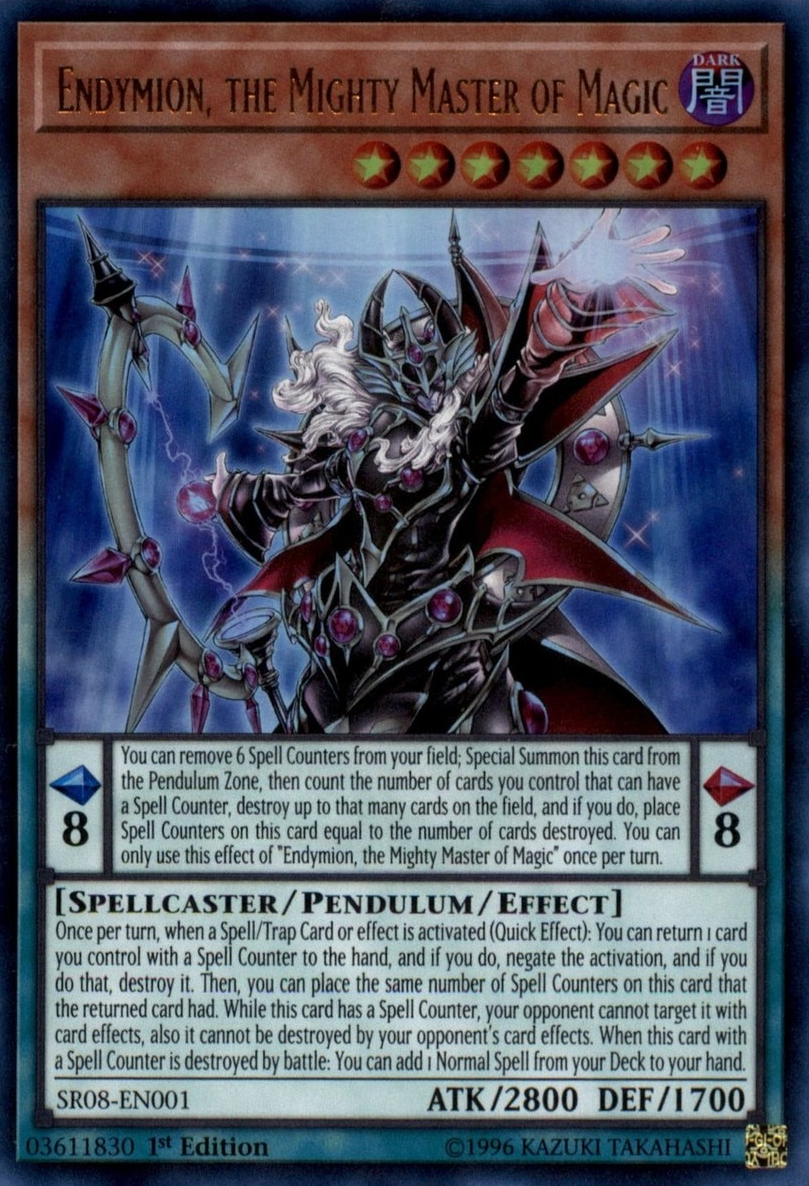
\includegraphics[width=.3\textwidth]{Abbildungen/Yu_Gi_Oh_card_example_with_a_lot_of_text.png}\hfill
	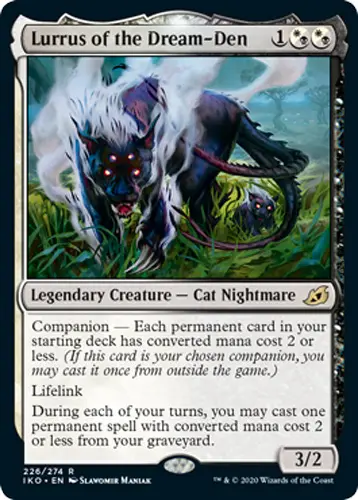
\includegraphics[width=.315\textwidth]{Abbildungen/Magic_the_gathering_card_example.png}\hfill
	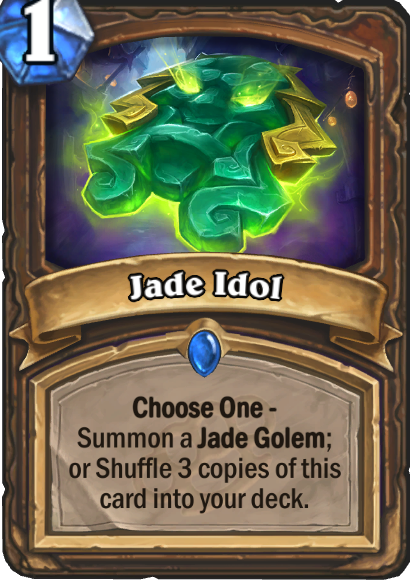
\includegraphics[width=.312\textwidth]{Abbildungen/Hearthstone_card_example_cropped.png}
	
	\caption{Beispiele für Sammelkarten}
	\label{fig:Examples_Of_Trading_Cards}
	
\end{figure}

\noindent Aber, obwohl das Rebranding von Sammelkarten zu Spielkarten ein Geniestreich war, hatte das Geschäftsmodell, wie es damals konzipiert wurde, drei Nachteile. Erstens, wenn das Unternehmen hinter der \ac{ip} Geld einnehmen wollte, musste es neue Karten drucken. Zweitens erschließt sich direkt aus Erstens. Wenn das Unternehmen hinter den Sammelkarten wollte, dass Kunden die neuen Karten kaufen, mussten die neuen Karten besser sein als die alten, was alte Karten und geliebte Spielstrategien, welche auf den alten Karten aufbauten, obsolet machte. Diese Entwicklung nennt man \glqq Power Creep\grqq. Dies führte dazu, dass neue Spieler die besseren Karten gerne kauften aber ältere Spieler entweder frustriert aufhörten, weil sie eine Strategie spielen wollten, die mit den neuen Karten nicht mithalten konnte, und zumindest Früher gab es neben \ac{mtg} keine Alternativen, oder sie bissen in den sauren Apfel und kaufen ebenfalls die neuen Karten, was auf emotionaler Ebene vielleicht noch schlimmer war, als einfach mit dem Spielen auf zu hören. Aber das schlimmste Problem des Geschäftsmodells war das moralische. Die Karten wurden nicht einfach verkauft, sie wurden, neben Starterpackungen, in Boosterpackungen verkauft. Boosterpackungen sind Packungen von 5-15 Karten verschiedener Seltenheit. Das heißt, dass besonders seltene Karten, besonders selten aus einer Boosterpackung gezogen werden. Wenn man aber doch eine besonders seltene Karte zieht, dann ist die Freude sehr groß -- genau wie bei einem Spielautomaten. Tatsächlich gibt es bereits Bestrebungen Lootboxen, die Computerspielversion von Boosterpackungen, rechtlich zu regulieren bzw. komplett zu verbieten. Es werden zusätzlich auch, in digitalen Versionen von Sammelkartenspielen, preisverschleiernde Mechaniken eingesetzt, um den Spieler zum Geldausgeben zu verführen. So kann man Karten nicht für Geld kaufen, sondern nur für eine intermediäre Währung, wie Kristalle. Kristalle werden aber nicht 1 zu 1 gegen Geld getauscht, sondern um einen Faktor, z.B. kriegt man für 10€ 1000 Kristalle und Karten kann man dann für 200 Kristalle kaufen. Das gewöhnt den Spieler große Mengen an Währung auszugeben und zu verschleiern, wie viel tatsächlich ausgegeben wurde. Es wird auch nie exakt so viel intermediäre verkauft wie man braucht. So kauft man 1000 Kristalle aber man braucht nur 700. Das führt dazu, dass immer Kristalle übrig bleiben und die Schwelle neue Kristalle zu kaufen niedriger wird, da man nicht so viele Kristalle braucht für einen neuen Kauf.\hfill\newline

%TODO rechtliche Sachen wegen Lootboxen rausfinden

\noindent Wir von Light Years Ahead - Gaming wollen diese drei Nachteile ausmerzen und, durch eine Weiterentwicklung des Geschäftsmodells, den Markt auf lange Sicht komplett einnehmen. Durch Verwenden des Business Model Canvas werden wir in dieser Seminararbeit das Geschäftsmodell Schritt für Schritt darlegen.  

\section{Markt} \label{sec:Markt}

Der Markt für Sammelkartenspiele ist seit seinen Anfängen in 1993 stark gewachsen und ist, für gedruckte Sammelkarten, im Jahr 2025 \$7.51Mrd groß und es wird erwartet, dass er bis zum Jahr 2030 auf \$10.98Mrd wächst~\cite{Print_TCG_Market_Size}. Auf der anderen Seite gibt es auch mittlerweile einen Markt für Online-Sammelkartenspiele. \ac{HS} allein hat zwischen 2014 und 2015 \$1Mrd eingebracht und der Markt selbst hatte in 2024 eine Größe von \$0.75Mrd und es wird erwartet, dass er auf in 2033 auf \$2.1Mrd wächst~\cite{Online_TCG_Market_Size}. Andere Quellen widersprechen aber diesen Zahlen. So wird in \cite{TCG_Market_Size_2024} angegeben, dass der globale Gesamtmarkt für Sammelkartenspiele, also analog und digital zusammen, im Jahr 2024 \$1Mrd betrug und es wird prognostiziert, dass er bis 2032 auf \$1.57Mrd wächst. In \cite{TCG_Market_Size} wird aber berichtet, dass der Gesamtmarkt im Jahr 2023 bereits einen Wert von \$7.6Mrd hatte und er soll bis 2032 sogar auf \$23.9Mrd wachsen. Wir entnehmen daraus, dass es einen Markt gibt und dass Gewinne, wie am Beispiel von \ac{HS}, realisiert werden können, wenn das Produkt gut genug ist.\hfill\newline

%TODO Heartstone Spielerzahlen rausfinden

\noindent Der Markt wird im Moment von den vier großen \acp{ip} beherrscht, die da wären \acl{mtg}, Yu-Gi-Oh, Pok\'emon und \acl{HS}. Dies sind aber nicht die größten Konkurrenten, da die Verantwortlichen hinter den \acp{ip} die \acp{ip} sehr schlecht behandeln. Die Kartenbeispiele in Abbildung~\ref{fig:Examples_Of_Trading_Cards} habe ich nicht zufällig gewählt. Diese drei Karten zeigen mindestens einen Aspekt auf, was mit dem momentanen Zustand der \acl{ip} falsch läuft. Die Karte ganz Links in Abbildung~\ref{fig:Examples_Of_Trading_Cards} ist aus Yu-Gi-Oh und wie man sehen kann ist der Effekttext extrem lang. Zu lang für neue Spieler. Abgesehen davon leidet Yu-Gi-Oh am stärksten unter dem ersten Nachteil des momentanen Geschäftsmodells. Wenn in Yu-Gi-Oh Karten gedruckt werden, dann werden gleich sehr viele Karten obsolet, was in einem starken Kaufzwang resultiert oder einer starken Abwanderung zu anderen Sammelkartenspielen. Die mittlere Karte ist aus \acl{mtg}. Das Problem hier ist nicht so offensichtlich aber es ist trotzdem schwerwiegend. Das Problem kommt aus dem Management von \ac{mtg}. Wie auf der Karte zu sehen, hat sie den Effekt \glqq Companion\grqq. In der Testphase für die neuen Karten mit diesem Effekt, wurde intern festgestellt, dass dieser Effekt zu stark ist und desaströs für den Spielspaß wäre. Aber trotz aller Warnungen haben die Verantwortlichen entschieden die Karten trotzdem raus zubringen, da sie sich große Gewinnen versprachen. Das Gegenteil ist eingetroffen und es musst das erste Mal seit 10 Jahren eine Regeländerung bekannt gegeben werden, damit das Spiel nicht komplett zerstört wird. Es würde über den Umfang dieser Seminararbeit gehen zu erklären, wieso die Karte ganz rechts schlecht für ihr Spiel war, aber wir können festhalten, dass sie so schlecht war, dass sie im Alleingang eine geliebte Spielstrategie von Heute auf Morgen ausgelöscht hat. Der größte Konkurrent ist \acl{fab}, da die Verantwortlichen hinter dieser \ac{ip} wenigstens eines der Nachtteile des Geschäftsmodells gelöst haben, das \glqq Power Creep\grqq, was \ac{fab} sehr erfolgreich gemacht hat. Aber wir wollen alles besser machen. Wie wird in Abschnitten~\ref{sec:Geschaeftidee} erläutert.

%TODO Zahlen zu FeB rausfinden und rausfinden, wo alles es besser gemacht wird, Kundensegmente? Erlösmodel?

\section{Geschäftsidee} \label{sec:Geschaeftidee}

Die Geschäftsidee beruht darauf alle Nachteile des bis dato dominierenden Geschäftsmodells auszumerzen. Dies wird erreicht, indem eine Software kreiert wird, mit deren Hilfe man Sammelkartenspiele erstellen kann, ohne auch nur eine Zeile Code geschrieben zu haben. Die Software besteht aus vier Editoren. Einen zu Erstellen des Spielfeldes und Zonen auf dem Spielfeld, in die Karten gelegt werden können, einen zum Erstellen von Karten und deren Interaktionen mit den Zonen und untereinander, einen zum Definieren von Zugphasen/-abschnitten, z.B. zum Definieren der Ziehphase oder Angriffsphase und einen zu Definieren/Organisieren von Turnieren. Ferner besteht die Software aus drei Marketplaces, einen für Bilder für Karten und Effekte, einen für Sounds und Musik, welche abgespielt werden, wenn man das Spiel startet oder eine Karte ausspielt und einen für Merchandise. Die Möglichkeit direkt aus der Software zu streamen ist ebenfalls ein Teil des Software.\hfill\newline

\noindent Das wichtigste Feature ist aber die Pitchen-und-Bewerten Mechanik. Gegeben ein Sammelkartenspiel, dass mit unserer Software erstellt wurde, kann jeder, der das Spiel installiert hat, eine Karte pitchen, also sich eine Karte ausdenken, sie mit dem Karteneditor verwirklichen und aus den Marketplaces entweder ein Bild und Sound/Musik kaufen oder leihen, und der Spielergemeinschaft die ausgedachte Karte zum Bewerten vorschlagen. Wenn man beim Pitchen sich etwas leiht, werden die Urheber des jeweiligen Bildes oder der jeweiligen Musik am Umsatz, den die Karte generiert, beteiligt. Wie die Beteiligung genau aussieht, wir im Abschnitt \glqq Erlösmodell\grqq{} erklärt. Die Bewertung erfolgt gewichtet. Dabei zählt die Stimme eines Spieler umso mehr, je länger er das gegebene Spiel gespielt hat und je höher sein Gewinn/Niederlage-Verhältnis ist. Dies garantiert, dass erfahrene Spieler eingreifen können, wenn eine schlechte Karte für das Spiel vorgeschlagen wird. Tatsächlich ist diese Mechanik so mächtig, dass generell keine Karten in das Spiel aufgenommen werden, die das Spiel nicht unmittelbar weiterbringen. Das bedeutet, dass diese Mechanik es unmöglich macht, neue Karten zu veröffentlichen, nur um Umsatz zu generieren. Wie wir trotzdem Umsatz generieren werden, wird näher in den Abschnitten \ref{sec:Kundensegmente} und \ref{sec:Erloesmodell} erläutert. Auf der anderen Seite garantiert die Pitchen-und-Bewerten Mechanik aber auch, dass ältere Karten und geliebte Spielstrategien erhalten bleiben und niemand in der Spielergemeinschaft frustriert wird, denn jede neue Karte bringt das Spiel weiter und das kann sie nur dann tun, wenn das, was vorher da war erhalten bleibt. Andererseits, da jede neue Karte das Spiel weiterbringt, wird mit jeder neuen Karte entweder eine ältere Strategie interessanter oder eine völlig neue Strategie erschaffen, was den Spaß für die Spielergemeinschaft nur steigert. Dies alles sorgt dafür, dass wir, im Gegenteil zu anderen \acp{ip}, keine Spieler verlieren, sondern nur neue dazugewinnen können. Somit werden wir den Markt auf lange Sicht einnehmen.\hfill\newline

\noindent Dies ist aber nur möglich, weil wir es geschafft haben alle (Sammel-)Kartenspiele auf wenige Grundmechaniken zu reduzieren. Zum Beispiel sind das Zerstören einer Karte, das Ziehen einer Karte und Ausspielen einer Karte oberflächlich drei verschiedene Interaktionen aber abstrahiert sind sie die selbe Interaktion, nämlich das Verschieben einer Karte von einer Zone in eine andere Zone. Das Zerstören einer Karte verschiebt die Karte von der Spielzone in die Ablagestapelzone, das Ziehen einer Karte verschiebt die Karte von der Kartenstapelzone in die Handzone und das Ausspielen einer Karte verschiebt die Karte aus der Handzone in die Spielzone. Alle anderen Interaktionen lassen sich ebenfalls auf Grundmechaniken reduzieren, die alle in einem der beiden Kataloge im Karteneditor gelistet sein werden. Der andere Katalog enthält bereits kombinierte Mechaniken, wie o.g. Zerstören, Ziehen und Ausspielen. Dies ermöglicht es neuen Karten intuitive zu erstellen, sodass jeder, der denkt, dass er eine gute Kartenidee hat, diese leicht pitchen kann. Damit aber es nicht zu einer Flut von Pitches für schlechten Karten kommt, integrieren wir zusätzlich die \glqq Fun-Measure-Funktion\grqq{} als Kontorllfeature. Die \glqq Fun-Measure-Funktion\grqq{} gibt an, wie viel Spaß eine Karte in das Spiel einbringt und ist ein unersetzliches Werkzeug für alle Spieler, die Teil des Wachstumsprozesses des Spiels sein wollen aber nicht so viel Erfahrung haben und besonders für \glqq Creator\grqq{} aus Abschnitt~\ref{subsubsec:Creator}, da diese davon Leben etwas zu erschaffen aber nicht die Erfahrung haben wie \glqq Hardcore Spieler\grqq{} aus Abschnitt~\ref{subsec:Hardcore_Spieler}.\hfill\newline

\noindent Für Spieler, die uns besonders stark unterstützen oder nur besonders stark angeben wollen, bieten wir zudem noch den \glqq Mensch-zu-Karte-Prozess\grqq{}. Das ist ein Prozess, den wir anbieten, gegen einen festen Preis, bei dem wir ein Photo von dem Spieler nehmen, es mit einer Bildbearbeitungssoftware bearbeiten und dann zusammen mit dem Spieler eine Karte machen, die vom Aussehen, allgemeiner Stärke und Effekt alle Beteiligten zufriedenstellen. Der Spieler kriegt im 50\% vom Gewinn, den wir durch den Verkauf der Karte erwirtschaften.

%TODO nachfragen, ob Grundinteraktionen und Fun-Measure-Funktion aufgeschrieben werden sollen

\noindent Schließlich entsagen wir auch der Spielautomaten-Mechanik durch Verkauf von Boosterpackungen und allen preisverscheiernden Mechaniken, da wir uns als \glqq The Good Guys \grqq positionieren wollen, ähnlich Larian Studios. Diese Positionierung ist wichtig, um das größte Kundensegment für uns zu gewinnen, wie im Abschnitt~\ref{sec:Kundensegmente} dargelegt wird.\hfill\newline

\noindent Wir ermöglichen es auch um Geld zu spielen und Gewinnanteile an Karten aus dem \glqq Mensch-zu-Karte-Prozess\grqq verkaufen.\hfill\newline

\noindent Um gleich uns als Gewinner zu etablieren, müssen wir sofort bei Veröffentlichung einschlagen und die positive Assoziation mit uns maximieren. Dies Erreichen wir, in dem wir sofort mit 3000 kostenlosen Karten starten, welche alle beliebten Spielstrategien abdecken und Monetarisierungswege anbieten, die sich gut anfühlen, wie im Abschnitt \glqq Erkömodell\grqq{} erläutert.\hfill\newline

\noindent Da wir darauf angewiesen sind, dass die Spieler unseres Spiels Karten pitchen, um das Spiel am Leben zu halten und es weiter zu entwickeln, 

\section{Kundensegmente} \label{sec:Kundensegmente}

Da wir unser Spiel zuerst digital anbieten, ergeben sich mehr und andere Kundensegmente, als wenn wir es im Print anbieten würden. Zwar ist das Ziel das Spiel nach mindestens 1Mio Spieler zusätzlich in den Print zu schicken aber, da das wahrscheinlich erst nach einem Jahr erreicht wird, konzentrieren wir uns zunächst auf die digitale Version.

\subsection{\acl{f2p} Spieler} \label{subsec:f2p_Spieler}

\acl{f2p} Spieler zeichnen sich durch zwei Eigenschaften aus. Die Eigenschaft ist, dass sie stur versuchen das Spiel kostenlos zu spielen, wenn das Spiel es ermöglicht. Und sollte das Spiel es nicht in einem angemessenen Zeitraum erlauben alle Inhalte komplett kostenlos zu erspielen, verlassen die \ac{f2p} Spieler die \ac{ip}. Da wir, wie im Anschnitt~\ref{sec:Erloesmodell} dargelegt, die Basisversionen jeder Karte kostenlos anbieten und gleichzeitig dafür sorgen, dass der Spielspaß unseres Spieles maximiert wird, wie im Abschnitt~\ref{sec:Geschaeftidee} beschrieben, garantieren wir, dass die \ac{f2p} Spieler in großen Zahlen bei uns bleiben und Spaß am Spiel haben. Dies ist notwendig, um das Kundensegment \glqq Wal\grqq, eines der beiden wichtigsten Kundensegmente, zu halten.\hfill\newline

\noindent Die zweite Eigenschaft, durch welche sich \ac{f2p} Spieler auszeichnen, ist, dass sie 70\%-90\% der Spieler von digitalen Spielen ausmachen. Kombiniert mit der Tatsache, dass \ac{f2p} Spieler es darauf anlegen Spiele kostenlos zu spielen, bedeutet es, dass der Großteil der Spielerbasis ausschließlich Kosten verursacht. Aber was andere Herausgeber von digitalen Sammelkartenspielen nicht realisiert haben ist, dass \ac{f2p} Spieler nichts ausgeben wollen, nicht weil sie es nicht wollen, sondern weil sie sich durch verschiedene Mechaniken, welche im Abshcnitt~\ref{sec:Einleitung} beschrieben werden, manipuliert fühlen. Und da die \ac{f2p} Spieler mit einem Teil des Spieles negative Gefühle verbinden, gerade dem Teil, der Umsatz generiert, fühlt es für sie schlecht an, Geld für das Spiel auszugeben. 

\subsubsection{Gelegenheitsspieler} \label{subsubsec:f2p_Spieler_Gelegenheitsspieler}

Dieses Kundensegment ist sehr klein aber, wie im Abschnitt~\ref{subsec:Wal} gezeigt, ist jeder Spieler wertvoll. \ac{f2p} Gelegenheitsspieler wollen nur gelegentlich Spielen, egal ob gegen unbekannte Spieler online oder gegen Freunde, das Spiel muss Spaß machen und am wichtigsten ist, dass das Spiel sich relativ nicht ändert. Das heißt, dass wenn der Spieler das Spiel an paar Monate nicht gespielt hat, keine neuen Karten raus gebracht wurden, die seine Karten und Spielstrategie obsolet machen. Gerade dieses Problem wird durch die Pitchen-und-Bewerten Mechanik behoben. Wir können also davon ausgehen, dass wir dieses Kundensegment, wenn einmal erreicht, halten können. Es muss aber betont werden, dass diese Spieler, selbst, wenn es sich für gut anfühlen würde Geld auszugeben, sie es wahrscheinlich nicht tun würden. Der einzige Grund, wieso wir dieses Kundensegment nicht komplett vernachlässigen, ist, dass wir für das Kundensegment \glqq Wal\grqq{} im Abschnitt~\ref{subsec:Wal} jeden Spieler brauchen.

\subsubsection{Kernspieler} \label{subsubsec:f2p_Spieler_Kernspieler}

Während Spieler im Abschnitt~\ref{subsubsec:f2p_Spieler_Gelegenheitsspieler}, wegen ihrer geringen Zahl, fast vernachlässigt werden können, machen \ac{f2p} Kernspieler 70\% bis 90\% aller Spieler in digitalen Sammelkartenspielen aus. Dies ist das \glqq \acl{f2p} Kernspieler-Problem\grqq. Und wir sind die einzigen, welche dieses Problem lösen können, da wir uns, wie im Abschnitt~\ref{sec:Geschaeftidee} beschrieben, als \glqq The Good Guys\grqq{} positionieren und unser Spiel so gestalten, dass es nicht nur Spaß macht es zu spielen, sondern es sich auch gut anfühlt für unser Spiel Geld auszugeben. Damit konvertieren wir mindestens 50\% der \ac{f2p} Kernspieler, was uns einen riesigen Wettbewerbsvorteil gegenüber unserer Konkurrenz liefert. Leider kann nicht genau angegeben werden, wie viel Umsatz dieses Kundensegment generiert, da bis jetzt es niemand geschafft hat es zu monetarisieren.

\subsection{Normale Spieler} \label{subsec:Normale_Spieler}

Normale Spieler sehen Sammelkartenspiele genauso wie alle anderen Beschäftigungen des Zeitvertreibs bzw. Hobbys. Sie sind bereit für ihr Hobby etwas zu bezahlen, haben jedoch kein Bedürfnis besonders gut darin zu werden oder viel Zeit in das Hobby zu investieren. Ansonsten sind sie identisch mit dem Kundensegment~\ref{subsubsec:f2p_Spieler_Gelegenheitsspieler}.

\subsubsection{Normaler Gelegenheitsspieler} \label{subsubsec:Normaler_Gelegenheitsspieler}

Normale Gelegenheitsspieler sind identisch zum Kundensegment~\ref{subsubsec:Normaler_Gelegenheitsspieler} mit dem Unterschied, dass sie eher bereit sind für ihren Zeitvertreib Geld auszugeben.

\subsubsection{Normaler Kernspieler} \label{subsubsec:Normaler_Kernspieler}

Normale Kernspieler sind identisch zum Kundensegment~\ref{subsubsec:f2p_Spieler_Kernspieler} mit dem Unterschied, dass sie eher bereit sind für ihren Zeitvertreib Geld auszugeben und, dass sie zahlenmäßig sehr viel weniger sind.

\subsection{Hardcore Spieler} \label{subsec:Hardcore_Spieler}

Hardcore Spieler wollen sich beweisen, sie wollen weniger Ruhm, sondern mehr ein Herausforderung. Sie studieren das Spiel um optimale Kartenkombinationen und beste Strategien zu entdecken. Man kann sie mit Profisportlern vergleichen, nur dass Hardcore Spieler nicht für Geld oder Ruhm spielen. Hardcore Spieler wollen vom Spiel Vielfalt, die wir liefern, da wir mit 3000 Karten starten. Sie wollen aber zudem ein Spiel, dass \glqq easy to learn, hard to master\grqq{} ist. Dies können wir auch zum Anfang mit den 3000 Karten garantieren. Abgesehen davon, dass in den initialen 3000 Karten herausfordernde Spielstrategien enthalten sein werden, kann jeder, der ein tieferes Verständnis vom Spiel hat, neue Karten und damit Spielstrategien pitchen, an die sonst niemand denken würde. Damit können Hardcore Spieler selbst dafür sorgen, dass für sie das Spiel nie zu langweilig wird, da sie dafür prädestiniert sind Karten am höchsten Level des Könnens zu erschaffen und dann zu spielen. Diese Gruppe ist wichtig, da, neben \glqq Creator\grqq{} in Abschnitt~\ref{subsubsec:Creator}, sie diejenigen sind, welche das Spiel vorantreiben und es interessant halten bzw. machen.

\subsection{Professionelle Spieler}

Professionelle Spieler, sind Spieler, die aus finanziellen Gründen und zum Teil für Ruhm, das Spiel spielen.

\subsubsection{Turnierspieler} \label{subsubsec:Professioneller_Spieler_Turnierspieler}

Turnierspieler sind Spieler, die auf Turniere gehen, um Geldpreise zu gewinnen. Das ist auch die einzige Klasse von professionellen Spielern, die auch zum Teil für Ruhm spielt. Diese Spieler sind wichtig, da sie diejenigen Spieler sind, welche man beim Spielen filmen kann und welche spannende Turniere ermöglichen, die ebenfalls gefilmt werden und veröffentlicht werden können. Bis jetzt sind spannende Turniere rar, da bis jetzt die Organisation eines Turniers mit großem Aufwand verbunden und selbst für Gruppen von Spielern zu teuer ist. Wir ändern das. Unsere Software, wie im Abschnitt~\ref{sec:Geschaeftidee} beschrieben, bietet intern sowohl die Möglichkeit mit ein paar wenigen Schritten ein Turnier aufzustellen als auch das Turnier direkt aus der Software heraus zu streamen.

\subsubsection{Onlinepokerspieler} \label{subsubsec:Professioneller_Spieler_Onlinepokerspieler}

Onlinepokerspieler bezeichnet hier die Klasse von Individuen, welche online an auf Können basierten Spielen teilnehmen mit dem Ziel Geld zu gewinnen. Solche Spiele können alles sein, sofern, auf lange Sicht, der bessere Spieler gewinnt. Zu solchen Spielen zählen u.a. Onlineschach und Onlinepoker selbst. Wenn aber ein Kunde dieses Segments etwas anderes als Schach oder Poker spielen wollte, gab es keine große Auswahl, insbesondere haben keine Sammelkartenspiele Funktionalitäten angeboten, um wie Onlinepoker gespielt zu werden. Unsere Software bietet genau das, denn man kann mit ihr um Geld spielen und Turniere zu veranstalten, wie in Onlinepoker. Leider kann nicht genau angegeben werden, wie viel Umsatz dieses Kundensegment generiert, da bis jetzt es niemand geschafft hat es zu monetarisieren.

\subsubsection{Streamer} \label{subsubsec:Professioneller Spieler_Streamer}

Streamer sind professionelle Spieler, die davon leben, dass es Spaß macht ihnen beim Spielen zuzuschauen. Bis jetzt ist das einzige Spiel, welches hinreichend schön anzusehen ist, ist \acl{HS}, aber eben nur hinreichend. Da wir einen dedizierten Marketplace haben für Bilder und Effekte, können Karten regelrecht absurde Effektvisualisationen haben, was sehr viel Spaß macht zuzuschauen. Da unser Spiel es aber auch ermöglicht sein Können zu zeigen, ist es optimal für Streamer.

\subsection{Wal} \label{subsec:Wal}

Vorneweg gesagt, wir finden die Bezeichnung \glqq Wal\grqq{} schlimm aber das ist leider Industriejargon. Abgesehen davon, bezeichnet \glqq Wal\grqq{} einen Kunden, der das Spiel nicht aus Spaß spielt, sondern nur, um damit anzugeben, dass er sich alles, was das Spiel bietet, leisten kann, je teurer, desto besser. In anderen Sammelkartenspielen kann man zwar kosmetische Verbesserungen für Karten kaufen aber es wird nichts angeboten, dass dieses Kundensegment direkt anspricht. Durch den \glqq Mensch-zu-Karte-Prozess\grqq{} sind wir die ersten, die dieses Kundensegment direkt monetarisieren. Ferner bieten wir für Karten, wie im Abschnitt~\ref{sec:Erloesmodell} beschrieben, besonders schön bearbeitete Bilder, rare Bilder, nur kurzzeitig verfügbare Bilder, besondere Kartenrücken, usw. an, welche direkt dieses Kundensegment als Ziel haben. Leider kann nicht genau angegeben werden, wie viel Umsatz dieses Kundensegment generiert, da bis jetzt es niemand geschafft hat es direkt zu monetarisieren.

\subsection{Kreative} \label{subsec:Kreative}

Als Kreative werden hier Menschen bezeichnet, die Freude empfinden, wenn sie etwas erschaffen, entweder einfach zum Spaß oder monetarisiert.

\subsubsection{Musiker/Künstler} \label{subsubsec:Musiker_Kuenstler}

Wie im Abschnitt~\ref{sec:Geschaeftidee} beschrieben, besitzt unsere Software einen dedizierten Marketplace für Bilder für Karten und Effekte und einen für Sounds und Musik. Wir werden aus Budgetgründen für die initialen 3000 Karten von KI generierte Bilder verwenden und der Musiker aus unserem Team macht die initialen Sounds und komponiert die erste Musik. Aber da wir uns als \glqq The Good Guys\grqq{} positionieren wollen, werden wir so früh es geht ausschließlich von Menschen gemalte Bilder nehmen. In unserem Marketplaces können Künstler und Musiker ihre Werke anbieten, um entweder direkt gekauft oder geliehen zu werden. Auch können die Musiker/Künstler im Marketplace für Merchandise ihre Produkte anbieten. Da Künstler und Musiker immer auf der Suche nach Möglichkeiten sind ihre Musik/Kunst/Merchandise zu verkaufen und wir einen Ort mit wenig Konkurrenz bieten, können wir mit hoher Partizipation rechnen. Der Vorteil für Musiker und Künstler bei uns ist auch, dass potenzielle Interessenten nicht explizit nach ihrer Musik/Kunst suchen müssen, da wir einen One-Stop-Shop liefern, wo sich Interessenten und Musiker/Künstler treffen können.\hfill\newline

\noindent Ein weiter Vorteil, den wir Musikern und Künstler bieten, ist, dass sie leicht jemanden zu finden, mit dem man kollaborieren kann, da Musiker, Künstler, Streamer, Fan-Creator und Wale an einem Ort sind.\hfill\newline

Diese Kundensegment wird nur indirekt monetarisiert, da das Anbieten von Kunst, Musik und Merchandise kostenlos ist und wir nur einen Anteil beim Verkauf bekommen.

\subsubsection{Fan-Creator} \label{subsubsec:Fan_Creator}

Dieses Kundensegment besteht auch Menschen, die es lieben etwas für ihr Hobby zu erschaffen. Im Fall von Sammelkartenspielen, sind das Menschen, die Sammelkarten zum Spaß erstellen. Sie veranstalten sogar kleine Wettbewerbe untereinander, wer die beste Karte zu ein einem vorgegebenen Thema macht. Ich war einer von ihnen. Und was aus heutiger Sicht frustrierend ist, ist die Tatsache, dass diese kreative Energie keiner der \ac{ip}-Holder interessiert. Die so entstandenen Karten werden nicht als Teil der \ac{ip} anerkannt und man kann mit ihnen in organisierten Veranstaltungen, von einer lockeren Runde im Spieleladen bis zum internationalen Turnier, nicht spielen. Die einzige Möglichkeit solche Karten zu spielen, ist im Freundeskreis aber das ist selten. Mittlerweile haben Influancer diese Bewegung aufgegriffen und mach Videos, in denen sie Fan-kreierte Karten vorstellen und bewerten.\hfill\newline

\noindent All dies ist den \ac{ip}-Holdern egal. Aber das ist nicht das erste Mal, dass so etwas passiert. Als Blizzard, die Computerspieleschmiede, Warcreaft III rausbrachte, haben Fans des Spiels eine Map von Warcraft III genommen und die Regeln so verändert, dass daraus ein komplett neues Spiel entstand. Diese Karte hieß \glqq \textbf{D}efense \textbf{o}f \textbf{t}he \textbf{A}ncients\grqq{} oder kurz DotA. DotA ist eingeschlagen, wie eine Bombe und wurde zum Hit. Aber das hat Blizzard nicht interessiert. Es gab weder monetären noch moralischen Support. Man konnte in DotA nichts kaufen oder verkaufen. Für DotA wurde keine Werbung gemacht und den Machern von DotA wurde auch keine Position in Blizzard angeboten, z.B. Senior Software Developer, welche ihren unglaublichen Erfolgt widerspiegeln würde. All das hat die Macher hinter DotA sehr verärgert und sie haben frustriert Riot gegründet und ein Konkurrenzprodukt raus gebracht, diese nannten sie \glqq \textbf{L}eague \textbf{o}f \textbf{L}egends\grqq{} oder kurt LOL. LOL wurde zu einem noch größeren Erfolg als DotA, sowohl wie es die Spielergemeinschaft aufnahm als auch monetär. Riot war wirtschaftlich extrem erfolgreich und 92.78\% wurde am 18 Februar 2011 von Tencent, dem chinesischen Softwaregiganten, für \$230Mio aufgekauft. Und erst als Blizzard gesehen hat, wie wirtschaftlich erfolgreich das Konzept ist, haben sie DotA Aufmerksamkeit geschenkt. Aber das war zu spät.\hfill\newline

\noindent Wir lernen aus den Fehlern anderer und haben auch deshalb die Pitchen-und-Bewerten eingeführt. Da man mit dieser Mechanik sogar neue Regeln entwerfen kann, können Fan-Creator in unserem Spiel komplett aufgehen.\hfill\newline

Leider kann nicht genau angegeben werden, wie viel Umsatz dieses Kundensegment generiert, da bis jetzt es niemand geschafft hat es zu monetarisieren. Mehr noch, dieses Kundensegment wird, wie oben beschrieben, aktiv ignoriert.

%TODO Geschichte von DOTA und dem Verbot von vanilla WoW

\subsection{Investoren} \label{subsec:Investoren}

\section{Erlösmodell} \label{sec:Erloesmodell}

Absolute Transparenz

Das Erlösmodell ist einfach. Wenn jemand mit unserer Software ein Spiel kreiert und Umsatz erzielt, nehmen wir 20\% des Umsatzes. Wenn in den Marketplaces etwas verkauft wird, verlangen wir auch hier 20\% des Umsatzes. 

10\% von Turnieren und pokerähnlichen Veranstaltungen

Wenn wir Umsatz generieren wollen, erlauben wir eine neue Reihe von Bildern für bereits bestehende Karten, anstatt neue Karten zu machen. Es können auch Sondereditionen erlaubt werden, wo Karten mehr kosten oder nur kurzzeitig verfügbare Bilder. Spieler haben das Gefühl uns zu unterstützen.

keine Slotmaschienen-Mechaniken durch Boosterpacks

% Literaturliste soll im Inhaltsverzeichnis auftauchen
\addcontentsline{toc}{section}{Literaturverzeichnis}

% Literaturliste endgueltig anzeigen
\bibliography{Literatur_Von_Der_Idee_zur_Gruendung.bib}

\newpage

\listoftables

\listoffigures

\newpage

\appendix

\addpart{Anlagen}

\pagenumbering{gobble}


\newpage

\begin{center}
	
	\fontsize{14pt}{12pt}
	
	\textbf{Erklärung}\\
	
\end{center}

\begin{verbatim}
	
	
	
\end{verbatim}

\noindent Ich versichere, dass ich die vorliegende Arbeit selbstständig und nur unter Verwendung der
angegebenen Quellen und Hilfsmittel angefertigt habe, insbesondere sind wörtliche oder
sinngemäße Zitate als solche gekennzeichnet. Mir ist bekannt, dass Zuwiderhandlung auch
nachträglich zur Aberkennung des Abschlusses führen kann.
Ich versichere, dass das elektronische Exemplar mit den gedruckten Exemplaren übereinstimmt.

\bigskip

\noindent\textbox{Ort: Leipzig\hfill}\textbox{\hfil Datum:\hfil}\textbox{\hfill Unterschrift:}

\end{document}